% VLSI LAB REPORT STRUCTURE TEMPLATE
% CREATED BY ISTIAK ALAM (CSE-20)
\documentclass[12pt,a4paper]{report}
\usepackage[utf8]{inputenc}
\usepackage[T1]{fontenc}
\usepackage{fontspec}
\setmainfont{Times New Roman}
\newfontfamily\hackfont{Hack}
\usepackage{titlesec}
\usepackage{fancyhdr}
\usepackage{listings}
\usepackage{xcolor}
\usepackage{graphicx}
\usepackage{longtable}
\usepackage{caption}
\usepackage{hyperref}
\usepackage{setspace}
\usepackage{geometry}
\geometry{a4paper, margin=1in}
\hypersetup{colorlinks=true, linkcolor=blue, urlcolor=blue}
\renewcommand{\contentsname}{Table of Contents}
\titleformat{\chapter}
  {\centering\Huge\bfseries}  % centering Chapter Name
  {Chapter \thechapter}               
  {1em}
  {} 


\begin{document}

% ---------------- COVER PAGE ----------------

\begin{titlepage}
\begin{center}
    
\includegraphics[width=0.35\textwidth]{assets/logo.png} \\
    \vspace{0.5cm}
    \textbf{\Huge \textcolor{cyan}{NOTRE DAME} \textcolor{cyan}{UNIVERSITY}} \\
    \vspace{0.5cm}
    \textbf{\Huge \textcolor{orange}{BANGLADESH}} \\

    \vspace{0.9cm}
    \textbf{\Huge \underline{Computer Graphics Lab Project Report}} \\

    \vspace{1.5em}
    \begin{flushleft} 
    	\textbf{\Large Course Code: CSE-4204} \\
		\vspace{0.3cm}
        \textbf{\Large Course Title: Computer Graphics Lab} \\
        \vspace{0.3cm}
        \textbf{\Large Project Title: Egg Drop Saga (Game)} \\
    \end{flushleft}

    \vspace{1em}
    \begin{flushleft}
        \textbf{\Huge \textcolor{blue}{Submitted by:}} \\
        \vspace{0.3cm}
        \textbf{\Large Name: Istiak Alam} \\
        \vspace{0.3cm}
        \textbf{\Large ID: 0692230005101005} \\
        \vspace{0.3cm}
        \textbf{\Large Name: Tanvir Hossain Ratul} \\
        \vspace{0.3cm}
        \textbf{\Large ID: 0692230005101004} \\
		\vspace{0.3cm}
        \textbf{\Large Batch: CSE-20} \\
        \vspace{0.5cm}
        \textbf{\Large Submission Date: }{\Large \textbf{\today}\par}
    \end{flushleft}

    \vfill
    \begin{flushleft}
        \textbf{\Huge \textcolor{blue}{Submitted to:}} \\
        \vspace{0.3cm}
        \textbf{\Large Humayara Binte Rashid} \\
        \vspace{0.3cm}
        \textbf{\Large Lecturer, Dept. of CSE} \\
        \vspace{0.3cm}
        \textbf{\Large Notre Dame University Bangladesh}
    \end{flushleft}

\end{center}
\end{titlepage}

% Table of Contents
\tableofcontents
\thispagestyle{empty}
\clearpage
\pagenumbering{arabic}

% Header Sections 
\pagestyle{fancy}
\fancyhf{} 							% Header Middle
\lhead{Computer Graphics Lab Project Report}
\rhead{Introduction}
\rfoot{\thepage}

\chapter*{\center Abstract}
\addcontentsline{toc}{chapter}{Abstract}
\thispagestyle{empty}

Egg Drop Saga is a 2D arcade-style game developed using OpenGL and GLUT in C++ as part of the Computer Graphics Laboratory course. The project demonstrates the practical application of fundamental computer graphics concepts including coordinate systems, geometric modeling, transformations, animation, rendering pipelines, and user interaction. In the game, a player controls a bucket to catch eggs dropped by moving chickens while avoiding missed catches that reduce the player's lives. The project incorporates real-time animation, keyboard-based controls, collision detection, score tracking, audio integration, and multiple game states such as menu, gameplay, pause, and game-over screens. The visual elements are created using OpenGL primitive drawing techniques and coordinate-based object construction. The primary objective of the project is to apply theoretical graphics concepts in an interactive environment while gaining experience in event-driven programming and real-time rendering. The final implementation successfully demonstrates the integration of computer graphics principles with game development techniques.


\chapter{Introduction}
%\addcontentsline{toc}{chapter}{Chapter-01 Introduction}


\section{Project Background}

Computer Graphics is a branch of computer science that focuses on the creation, manipulation, and rendering of visual content using computational techniques. OpenGL is one of the most widely used graphics libraries for developing interactive graphical applications and games. As part of the Computer Graphics Laboratory course, students are encouraged to apply theoretical concepts such as coordinate systems, geometric modeling, transformations, animation, rendering, and event handling in a practical project.\\

The project \textbf{Egg Drop Saga} is a 2D arcade-style game developed using C++ and OpenGL (GLUT). The game simulates a farm environment where chickens continuously move and drop eggs from the top of the screen. The player controls a bucket positioned at the bottom of the screen and must catch the falling eggs to earn points while avoiding missed catches that reduce the player's lives. The project integrates graphical object modeling, real-time animation, collision detection, user interaction, and audio feedback into a complete gaming experience.

\section{Motivation}

The inspiration for this project came from classic arcade catching games that emphasize quick reaction and hand-eye coordination. These games are simple in design yet provide an engaging user experience through continuous movement, scoring systems, and increasing difficulty. \\

From an academic perspective, the project offered an opportunity to implement various computer graphics concepts learned throughout the course in a practical environment. Developing a complete game using OpenGL allowed the team to gain hands-on experience with rendering pipelines, object-oriented design, animation techniques, coordinate-based drawing, and event-driven programming while creating an enjoyable interactive application.

\newpage
\section{Objectives}
The primary objectives of the Egg Drop Saga project are:

\begin{itemize}
\item To develop a fully functional 2D game using OpenGL and GLUT.

\item To understand and implement the OpenGL rendering pipeline.

\item To apply coordinate-based geometric modeling for creating game objects such as chickens, eggs, buckets, and backgrounds.

\item To implement real-time animation for moving objects within the game environment.

\item To develop keyboard-based user interaction for controlling game elements.

\item To implement collision detection between falling eggs and the player's bucket.

\item To create a score and life management system.

\item To integrate sound effects and background music for enhanced gameplay.

\item To gain practical experience in object-oriented game development using C++.


\end{itemize}

\section{Scope}

The scope of the project includes the design and implementation of a complete 2D arcade game using OpenGL. The project covers graphical object creation, rendering, animation, collision detection, score management, sound integration, and user interaction through keyboard controls.\\

The game contains multiple functional components including a main menu, gameplay screen, pause system, score tracking, life management, and game-over interface. All visual elements are generated using OpenGL primitives and coordinate-based drawing techniques rather than external game engines.\\

However, the project does not include advanced features such as 3D graphics, online multiplayer support, artificial intelligence opponents, physics engines, networking systems, or database integration. The focus remains on demonstrating core computer graphics principles within a 2D interactive environment.







\newpage
\chapter{System Design}
\rhead{System Design}


\section{System Overview}

Egg Drop Saga is implemented using an event-driven architecture based on OpenGL and GLUT. The system is organized around a central \texttt{Game} class that manages gameplay logic, rendering operations, collision detection, animation updates, score management, and state transitions.\\

The application begins execution from \texttt{main.cpp}, where the OpenGL environment, GLUT window, audio system, and callback functions are initialized. Once initialization is complete, GLUT takes control through its event loop and continuously invokes registered callback functions.\\

The overall execution flow is shown below:

\begin{figure}[h]
    \centering
    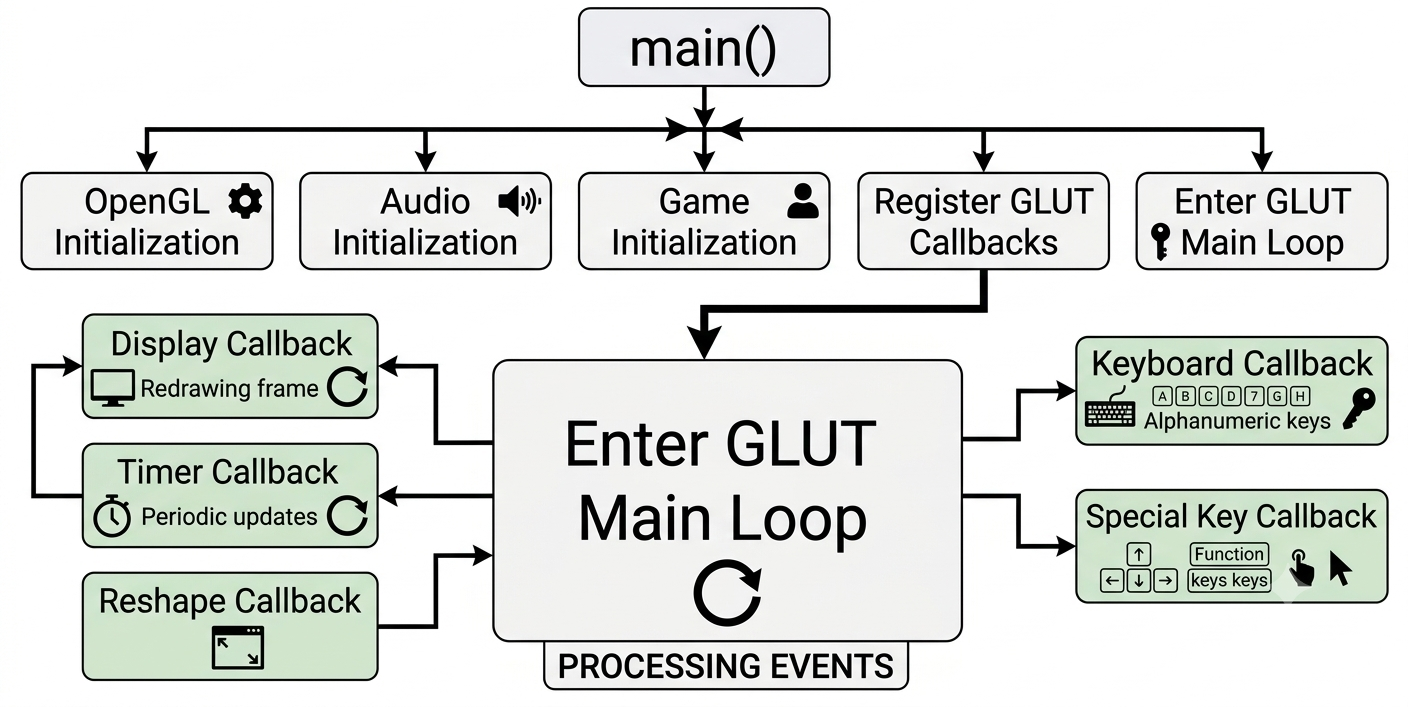
\includegraphics[width=0.9\textwidth]{assets/system overview.png}
    \caption{Application Initialization}
\end{figure}

The system continuously updates and renders the game at approximately 60 frames per second using a timer-based animation loop.

\newpage
\section{Game State Management}

The game operates using a finite state machine (FSM) implemented through the \texttt{GameState} enumeration.

\begin{verbatim}
enum GameState
{
HOME,
PLAYING,
GAME_OVER
};
\end{verbatim}

The state transitions occur as follows:

\begin{figure}[h]
    \centering
    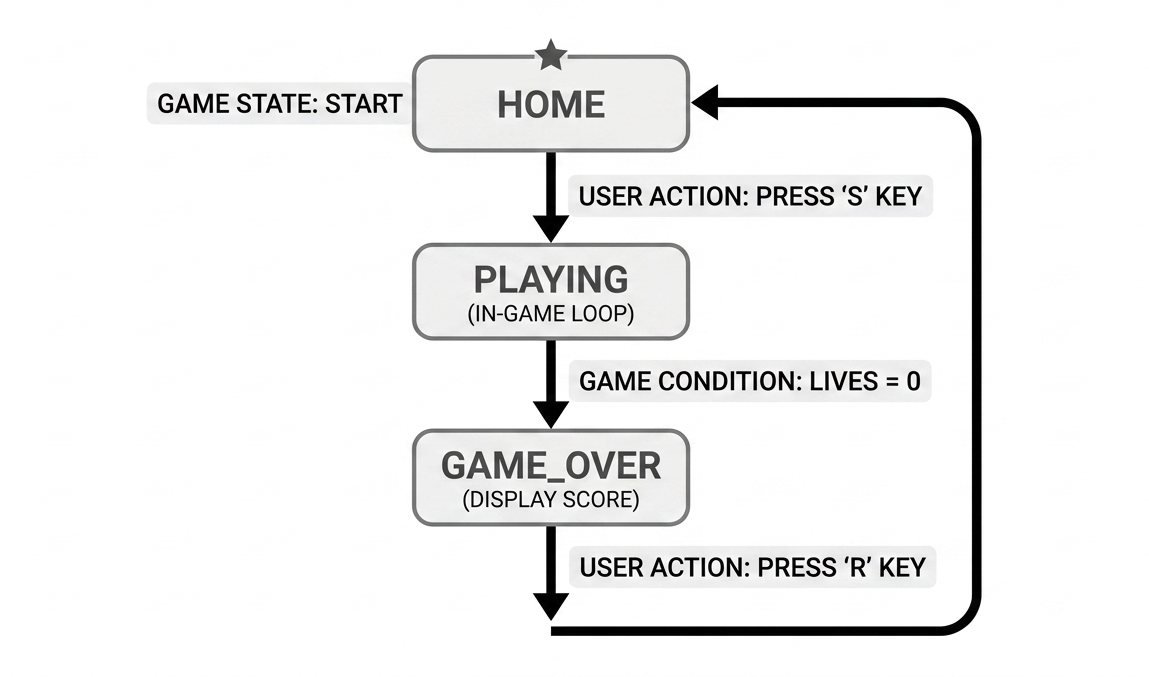
\includegraphics[width=0.9\textwidth]{assets/Game-state.png}
    \caption{Game State Transition}
\end{figure}

This approach simplifies gameplay management by ensuring that only the logic associated with the active state is executed.


\section{OpenGL Rendering Pipeline}

The rendering process of Egg Drop Saga follows a structured pipeline that is executed repeatedly during gameplay.

\subsection*{Stage 1: Initialization}

During program startup, the following operations are performed:

\begin{itemize}
\item GLUT initialization using \texttt{glutInit()}.
\item Creation of the game window.
\item Activation of RGB color mode.
\item Activation of double buffering.
\item Configuration of alpha blending.
\item Setup of the orthographic projection.
\item Initialization of game resources.
\item Loading of audio files.
\end{itemize}

\subsection*{Stage 2: Input Processing}

Player input is captured through GLUT callback functions.

\begin{itemize}
\item \texttt{keyboard()} handles standard keyboard input.
\item \texttt{specialKeys()} handles arrow key input.
\end{itemize}

The input is forwarded to:

\begin{verbatim}
game.handleInput()
game.handleSpecialInput()
\end{verbatim}

These functions update the bucket position, game state, pause state, and audio settings.

\subsection*{Stage 3: Update Cycle}

The timer callback executes every 16 milliseconds.

\begin{verbatim}
glutTimerFunc(16, timer, 0);
\end{verbatim}

This produces approximately:\\


$FPS = \frac{1000}{16}
\approx 60$\\


During each update cycle:

\begin{itemize}
\item Background animation is updated.
\item Home screen animation is updated.
\item Eggs are spawned if necessary.
\item Egg positions are updated.
\item Collision detection is performed.
\item Score and life counters are updated.
\end{itemize}

\subsection*{Stage 4: Rendering}

The display callback invokes:

\begin{verbatim}
game.render();
\end{verbatim}

The rendering order is:

\begin{enumerate}
\item Clear frame buffer.
\item Draw background.
\item Draw chickens.
\item Draw eggs.
\item Draw bucket.
\item Draw score text.
\item Draw life indicators.
\item Draw state-specific screens.
\end{enumerate}

\subsection*{Stage 5: Buffer Swapping}

After rendering completes:

\begin{verbatim}
glutSwapBuffers();
\end{verbatim}

The back buffer becomes visible while the next frame is rendered in the hidden buffer.

This double-buffering technique eliminates screen flickering and ensures smooth animation.


\section{Coordinate System Design}

Egg Drop Saga uses a two-dimensional orthographic coordinate system configured through:

\begin{verbatim}
gluOrtho2D(0, GAME_WIDTH, 0, GAME_HEIGHT);
\end{verbatim}

The coordinate system is defined as follows:

\begin{itemize}
\item Origin (0,0) is located at the bottom-left corner.
\item Positive X values extend toward the right.
\item Positive Y values extend upward.
\item All game objects are positioned using world coordinates.
\end{itemize}
  
\begin{figure}[!h]
    \centering
    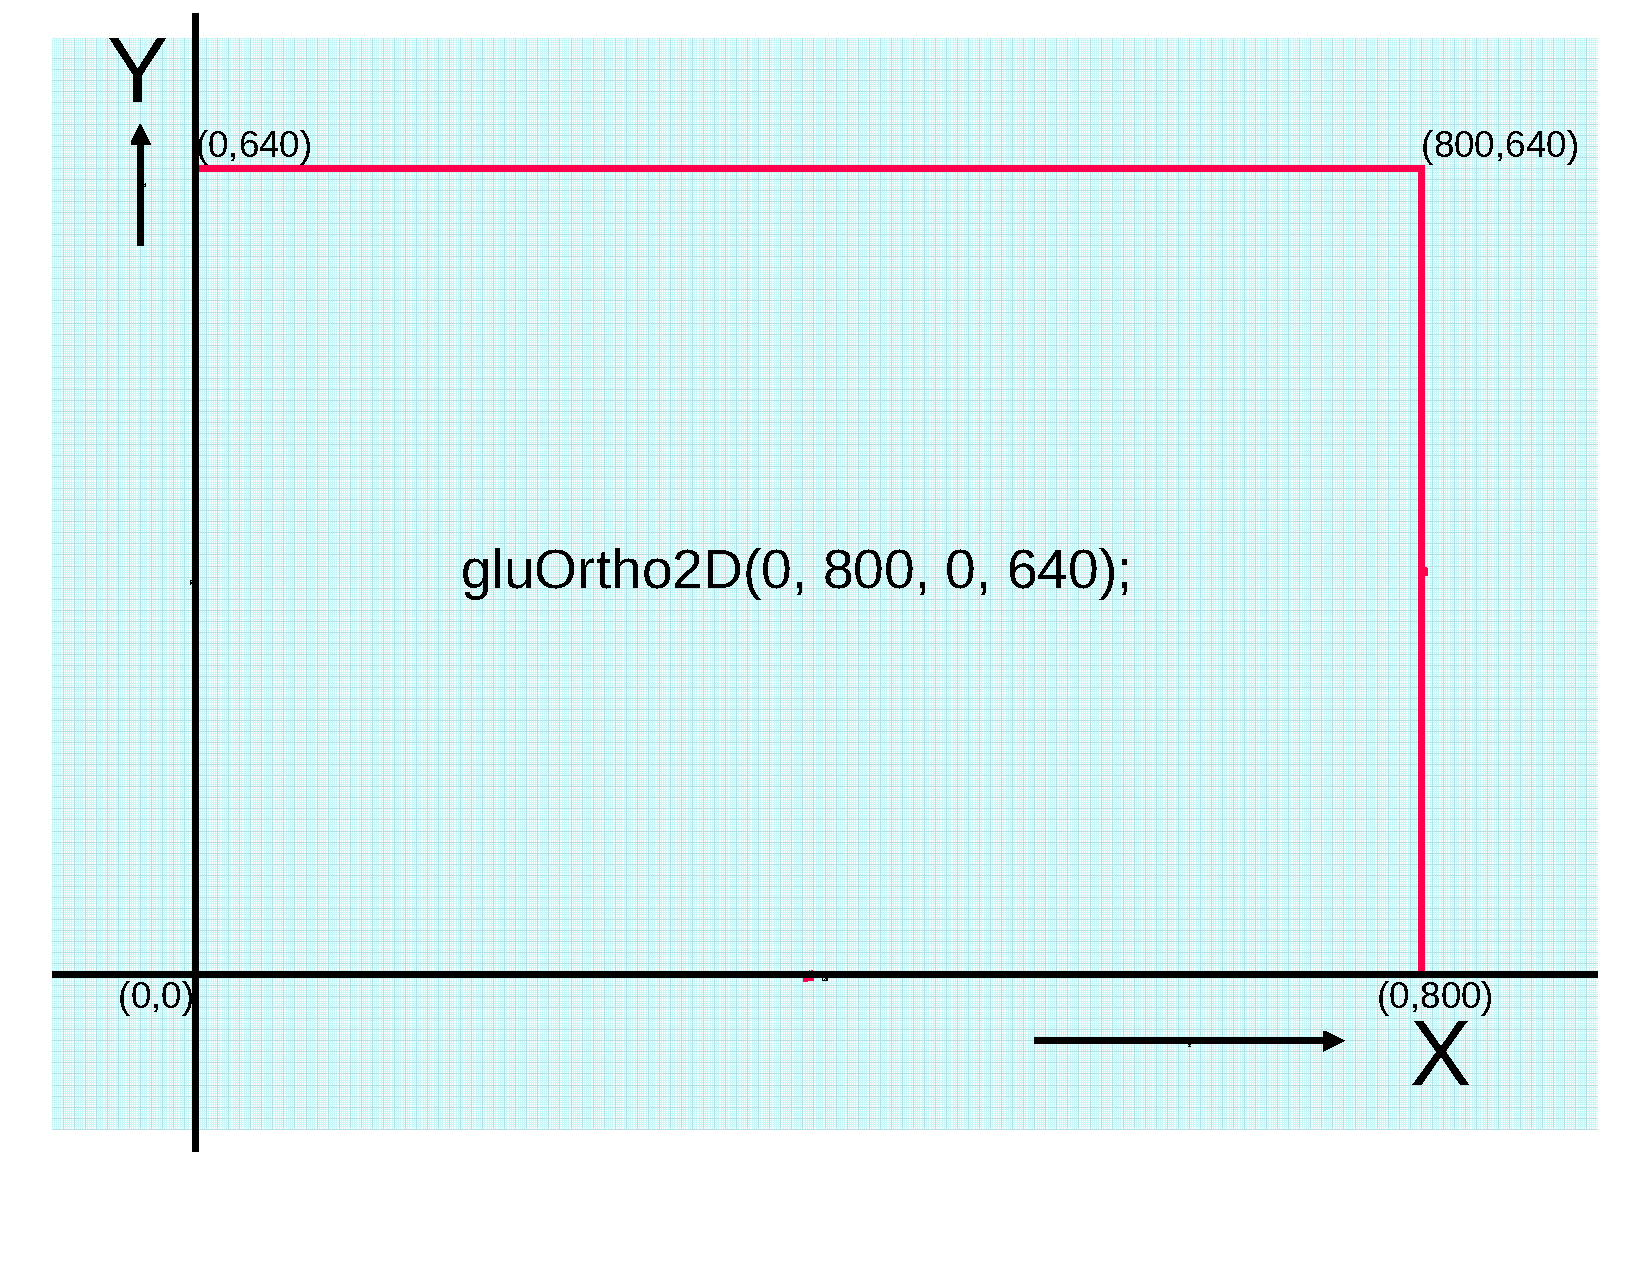
\includegraphics[width=1\textwidth]{assets/glOrthopdf.pdf}
    \caption{orthographics Graph of the Game Screen}
\end{figure}

Examples of object positioning:

\begin{itemize}
\item Bucket is initialized near the bottom of the screen.
\item Chickens are positioned along the upper wire.
\item Eggs spawn below randomly selected chickens.
\item UI elements are positioned using fixed coordinates.
\end{itemize}


\section{Component Description}

The Egg Drop Saga game is composed of several independent modules. Each module is responsible for a specific functionality and collectively contributes to the complete gameplay experience.

\subsection*{Game Module}

The \texttt{Game} class acts as the central controller of the application.

Responsibilities include:

\begin{itemize}
\item Managing game states (Home, Playing, Game Over)
\item Updating game objects
\item Rendering all scene components
\item Handling collision detection
\item Maintaining score and life counters
\item Coordinating audio playback
\end{itemize}

The Game class serves as the communication bridge between all other modules.

\subsection*{Chicken Module}

The Chicken module represents the chickens positioned near the top portion of the game screen.

Main responsibilities:

\begin{itemize}
\item Maintaining chicken positions
\item Rendering chicken graphics
\item Providing egg spawning locations
\end{itemize}

Five chickens are created during game initialization and distributed evenly along the upper wire.

The chicken model is constructed using primitive OpenGL shapes including:

\begin{itemize}
\item Circular body
\item Circular head
\item Elliptical neck
\item Polygon wing
\item Tail feathers
\item Comb
\item Beak
\item Legs
\end{itemize}

Transformation operations such as translation and rotation are applied to position body parts correctly.

\subsection*{Egg Module}

The Egg module controls the falling eggs and their associated animations.

Responsibilities include:

\begin{itemize}
\item Egg generation
\item Vertical movement
\item Ground collision handling
\item Squash animation
\item Broken egg rendering
\item Shadow generation
\end{itemize}

The egg transitions through three states:

\begin{enumerate}
\item Falling State
\item Squashing State
\item Broken State
\end{enumerate}

This creates a more realistic visual effect compared to immediate disappearance after ground impact.

\subsection*{Bucket Module}

The bucket serves as the player-controlled object.

Responsibilities include:

\begin{itemize}
\item Horizontal movement
\item Collision detection
\item Catching eggs
\item Boundary restriction
\end{itemize}

The bucket is drawn using:

\begin{itemize}
\item Semi-elliptical basket body
\item Gradient shading
\item Curved outlines
\item Decorative weave patterns
\item Ground shadow
\end{itemize}

Movement is restricted within the game boundaries to prevent the bucket from leaving the visible play area.

\subsection*{Background Module}

The Background module draws the complete game environment.

Responsibilities include:

\begin{itemize}
\item Sky rendering
\item Ground rendering
\item Environmental decorations
\item Animated scenery
\end{itemize}

This layer is rendered before all gameplay objects to create proper depth ordering.

\subsection*{AudioManager Module}

The AudioManager module handles all sound effects and music.

Responsibilities include:

\begin{itemize}
\item Loading audio files
\item Playing background music
\item Playing sound effects
\item Managing audio volume
\end{itemize}

Separate audio tracks are used for:

\begin{itemize}
\item Home Screen Music
\item Gameplay Music
\item Game Over Music
\item Egg Catch Effect
\item Egg Break Effect
\item Chicken Sound Effect
\end{itemize}

\section{Transformation and Animation Logic}

The project uses several geometric transformations to create movement and animation effects.

\subsection*{Translation}

Translation is the most frequently used transformation in the project.

The general translation equation is:


$P'(x,y)=(x+t_x,;y+t_y)$


where:

\begin{itemize}
\item $P(x,y)$ is the original point.
\item $P'(x,y)$ is the translated point.
\item $t_x$ and $t_y$ represent displacement values.
\end{itemize}

\paragraph{Chicken Translation}

Each chicken is positioned using:

\begin{verbatim}
glTranslatef(x, y, 0);
\end{verbatim}

This moves the chicken model from the origin to its assigned position on the wire.

\paragraph{Egg Translation}

The egg falls downward by continuously decreasing its y-coordinate.


$y_{new}=y_{old}-speed$


As the game score increases, egg speed also increases, increasing game difficulty.

\paragraph{Bucket Translation}

The bucket moves horizontally according to keyboard input.


$x_{new}=x_{old}\pm speed$


where:


$speed=50$


Boundary checks ensure that the bucket remains within the visible game area.


\subsection*{Scaling}

Scaling is used during the egg squash animation.

The transformation is implemented as:

\begin{verbatim}
glScalef(scaleX, scaleY, 1.0f);
\end{verbatim}

When the egg hits the ground:

\begin{itemize}
\item Vertical scale decreases.
\item Horizontal scale increases.
\end{itemize}

This creates a realistic squash-and-stretch effect commonly used in animation principles.

\section{Collision Detection Mathematics}

Collision detection is implemented between the bucket and the falling egg.

The collision condition is:


$Egg_X > Bucket_X$


and

$
Egg_X < Bucket_X + Bucket_{Width}
$

and

$
Egg_Y - Radius < Bucket_Y + Bucket_{Height}
$

If all conditions are satisfied simultaneously, the egg is considered successfully caught.

The actual implementation is:

\begin{verbatim}
return (egg.x > x &&
egg.x < x + width &&
egg.y - egg.radius < y + height);
\end{verbatim}

When a collision occurs:

\begin{itemize}
\item Catch sound effect is played.
\item Score increases by one.
\item Current egg is removed.
\item A new egg is generated.
\end{itemize}

\section{Object Lifecycle}

The lifecycle of an egg is illustrated below:

\begin{figure}[h]
    \centering
    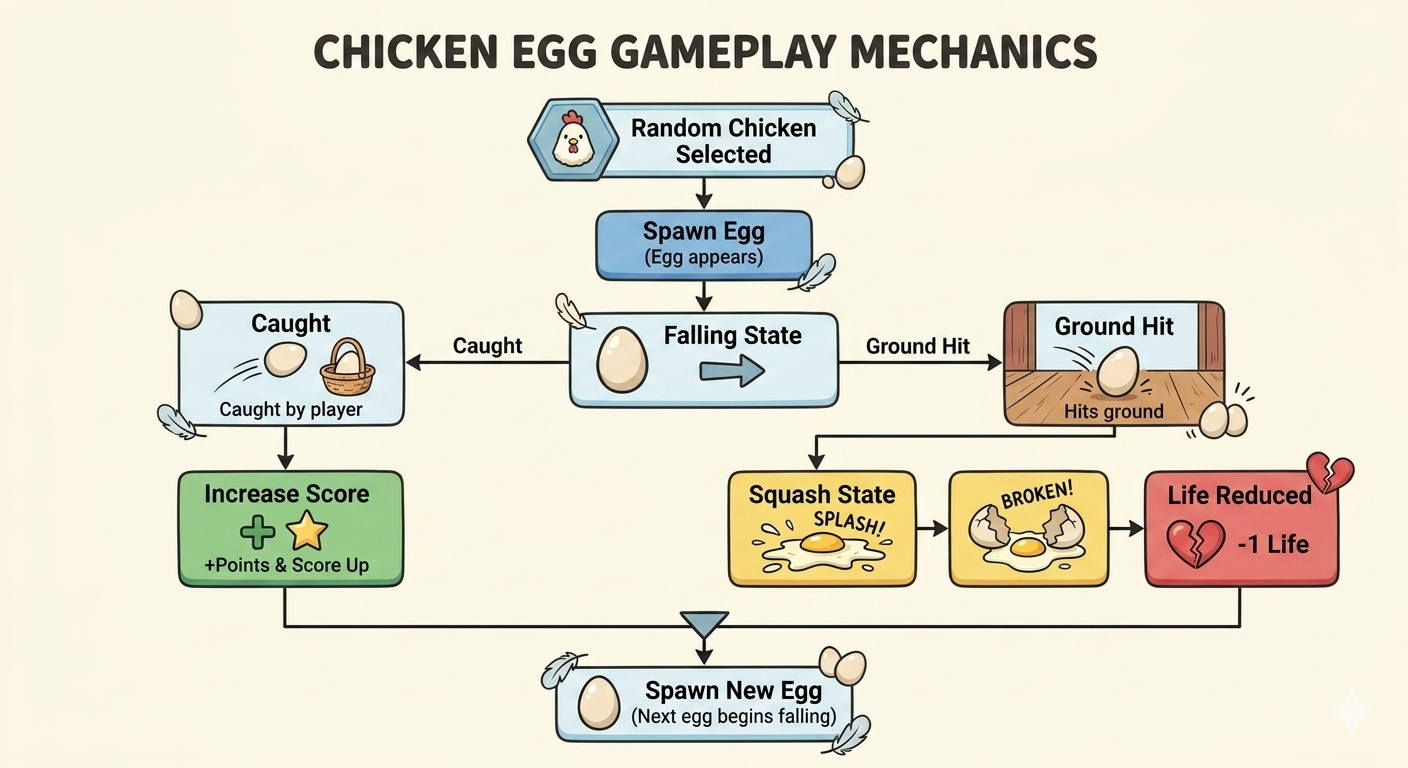
\includegraphics[width=0.9\textwidth]{assets/Egg lifecycle.png}
    \caption{Egg Life Cycle}
\end{figure}

This lifecycle governs the complete gameplay mechanics and ensures continuous interaction between the player and falling objects.

\section{OpenGL Drawing Primitives Used}

The graphical objects in Egg Drop Saga are constructed entirely using OpenGL's immediate mode rendering primitives. Complex game objects such as chickens, eggs, buckets, shadows, and user interface elements are created by combining multiple geometric primitives.

The project demonstrates practical applications of fundamental computer graphics concepts including polygon modeling, curve approximation, transformations, shading, and animation.

\subsection*{GL\_TRIANGLE\_FAN}

The \texttt{GL\_TRIANGLE\_FAN} primitive is the most frequently used primitive in the project.

It constructs a series of connected triangles sharing a common center vertex, making it ideal for creating circular and curved shapes.

\textbf{Applications in the Project:}

\begin{itemize}
\item Chicken body
\item Chicken head
\item Chicken tail feathers
\item Chicken comb
\item Egg body
\item Egg highlights
\item Egg shadow
\item Broken egg splash
\item Bucket body
\item Heart icons (life indicators)
\end{itemize}

Example implementation:

\begin{verbatim}
glBegin(GL_TRIANGLE_FAN);
glVertex2f(centerX, centerY);

for(int i=0; i<=60; i++)
{
float angle = 2*PI*i/60;
glVertex2f(
centerX + radius*cos(angle),
centerY + radius*sin(angle)
);
}
glEnd();
\end{verbatim}

This technique approximates circles and ellipses by connecting multiple vertices around a central point.

\subsection*{GL\_POLYGON}

The \texttt{GL\_POLYGON} primitive is used to create filled irregular shapes composed of multiple connected vertices.

\textbf{Applications in the Project:}

\begin{itemize}
\item Chicken wing geometry
\end{itemize}

Example:

\begin{verbatim}
glBegin(GL_POLYGON);
...
glEnd();
\end{verbatim}

This primitive allows the creation of more organic shapes that cannot be represented using simple rectangles or circles.

\subsection*{GL\_TRIANGLES}

The \texttt{GL\_TRIANGLES} primitive is used to create individual triangular shapes.

\textbf{Applications in the Project:}

\begin{itemize}
\item Chicken beak
\end{itemize}

Example:

\begin{verbatim}
glBegin(GL_TRIANGLES);
glVertex2f(...);
glVertex2f(...);
glVertex2f(...);
glEnd();
\end{verbatim}

The triangular beak provides a simple yet effective representation of the chicken's facial features.

\subsection*{GL\_QUADS}

The \texttt{GL\_QUADS} primitive is used to create rectangular surfaces using four vertices.

\textbf{Applications in the Project:}

\begin{itemize}
\item Ground platform
\item Grass layer
\item Basket rim
\item User interface panels
\end{itemize}

Example:

\begin{verbatim}
glBegin(GL_QUADS);
glVertex2f(x1,y1);
glVertex2f(x2,y2);
glVertex2f(x3,y3);
glVertex2f(x4,y4);
glEnd();
\end{verbatim}

Quadrilaterals are efficient for constructing flat surfaces and environmental elements.

\subsection*{GL\_LINES}

The \texttt{GL\_LINES} primitive is used for rendering independent line segments.

\textbf{Applications in the Project:}

\begin{itemize}
\item Chicken legs
\item Chicken toes
\item Basket weaving pattern
\end{itemize}

Example:

\begin{verbatim}
glBegin(GL_LINES);
glVertex2f(x1,y1);
glVertex2f(x2,y2);
glEnd();
\end{verbatim}

These line segments provide additional visual details without significantly increasing rendering complexity.

\subsection*{GL\_LINE\_LOOP}

The \texttt{GL\_LINE\_LOOP} primitive creates a closed outline by automatically connecting the last vertex back to the first vertex.

\textbf{Applications in the Project:}

\begin{itemize}
\item Egg outline
\item Chicken body outline
\item Chicken head outline
\item Chicken comb outline
\item Chicken beak outline
\item Tail feather outlines
\item Basket rim outline
\item Broken egg components
\end{itemize}

Example:

\begin{verbatim}
glBegin(GL_LINE_LOOP);
...
glEnd();
\end{verbatim}

The use of outlines improves object visibility and visual separation between adjacent shapes.

\subsection*{GL\_LINE\_STRIP}

The \texttt{GL\_LINE\_STRIP} primitive draws a continuous connected sequence of lines.

\textbf{Applications in the Project:}

\begin{itemize}
\item Basket curved outline
\item Wing feather details
\end{itemize}

Example:

\begin{verbatim}
glBegin(GL_LINE_STRIP);
...
glEnd();
\end{verbatim}

This primitive is useful for representing curved boundaries and decorative details.

\section{Graphics Techniques Implemented}

In addition to primitive-based modeling, several graphics techniques were incorporated to improve the visual quality of the game.

\subsection*{Gradient Shading}

Gradient shading is used extensively throughout the project.

Examples include:

\begin{itemize}
\item Egg surface shading
\item Bucket body shading
\item Heart icons
\item Egg yolk rendering
\end{itemize}

Different vertex colors are assigned to neighboring vertices, allowing OpenGL to interpolate colors smoothly across the surface.

\subsection*{Alpha Blending}

Transparency effects are implemented using OpenGL blending.

\begin{verbatim}
glEnable(GL_BLEND);
glBlendFunc(GL_SRC_ALPHA,
GL_ONE_MINUS_SRC_ALPHA);
\end{verbatim}

Applications include:

\begin{itemize}
\item Egg shadows
\item Bucket shadows
\item Egg highlights
\end{itemize}

This technique creates smoother and more realistic visual effects.

\subsection*{Shadow Rendering}

Dynamic shadows are generated beneath falling eggs and the bucket.

The shadow size changes according to the object's height above the ground.

As the egg falls:

\begin{itemize}
\item Shadow becomes smaller.
\item Shadow becomes darker.
\end{itemize}

This creates an illusion of depth in the two-dimensional environment.

\subsection*{Squash and Stretch Animation}

The project implements the classical animation principle of squash and stretch.

When an egg reaches the ground:

\begin{itemize}
\item Vertical scale decreases.
\item Horizontal scale increases.
\end{itemize}

This transformation produces a more natural and visually appealing impact animation before the egg breaks.

\subsection*{Double Buffering}

To eliminate rendering flicker, the project uses OpenGL double buffering.

\begin{verbatim}
glutInitDisplayMode(
GLUT_DOUBLE | GLUT_RGB
);
\end{verbatim}

After each frame is rendered:

\begin{verbatim}
glutSwapBuffers();
\end{verbatim}

The back buffer becomes visible while rendering continues in the hidden buffer.

This ensures smooth animation and stable frame presentation.



This chapter presented the complete system design of Egg Drop Saga. The overall architecture, component interactions, rendering pipeline, coordinate system, object lifecycle, animation techniques, collision detection algorithms, and OpenGL primitives were discussed in detail. The implementation demonstrates practical applications of fundamental computer graphics concepts including geometric modeling, transformations, shading, animation, event-driven programming, and real-time rendering using OpenGL and GLUT.




\chapter{Implementation}
\rhead{Implementation}
\section{Implementation}

This chapter describes the practical implementation of the Egg Drop Saga game using C++, OpenGL, GLUT, and SDL2\_mixer. It explains the development environment, implementation process, integration of modules, and important code segments used to create the final application.

\section{Tools and Development Environment}

The development of Egg Drop Saga required several software tools and libraries, which are listed below:

\begin{table}[!h]
\centering

\begin{tabular}{|p{4cm}|p{8cm}|}
\hline
\textbf{Tool/Library} & \textbf{Purpose} \\
\hline
C++ & Primary programming language used for game development. \\
\hline
OpenGL & Graphics rendering library used for drawing and displaying visual objects. \\
\hline
GLUT (OpenGL Utility Toolkit) & Provides window management, event handling, keyboard input, and rendering callbacks. \\
\hline
SDL2\_mixer & Used for audio playback including background music and sound effects. \\
\hline
Code::Blocks & Integrated Development Environment (IDE) used for coding and debugging. \\
\hline
MinGW GCC Compiler & Compiles and links the C++ source code. \\
\hline
Windows Operating System & Development and testing platform. \\
\hline
GitHub & Version control and project collaboration. \\
\hline
\end{tabular}
\caption{Tools and Libraries}
\end{table}


The graphics subsystem was implemented using OpenGL's immediate mode rendering functions. GLUT was used to manage windows, user input, and event callbacks, while SDL2\_mixer provided support for background music and sound effects.

\section{Project Structure}

The Egg Drop Saga project follows a modular object-oriented architecture where each major game component is implemented as an independent class. This design improves code maintainability, readability, and scalability by separating rendering, game logic, audio management, and user interface functionalities into distinct modules.\\

The overall project directory structure is shown below:


\begin{figure}[h]
    \centering
    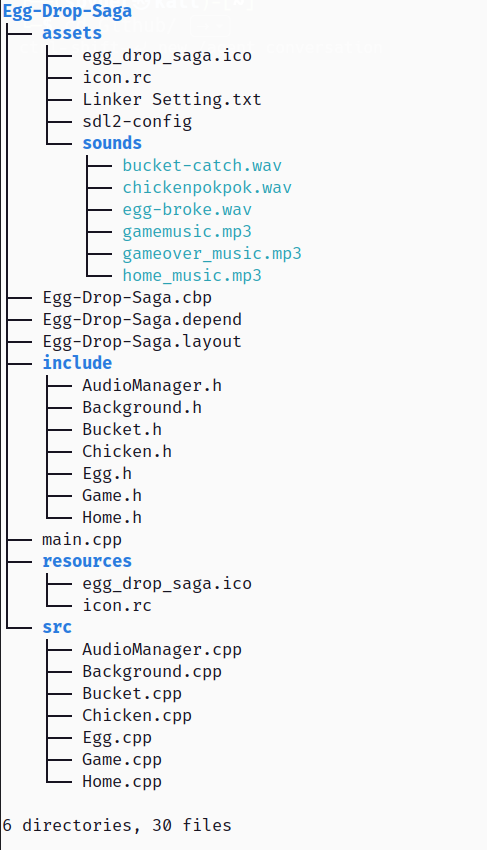
\includegraphics[width=0.6\textwidth]{assets/project-structure.png}
    \caption{Project File Structure}
\end{figure}



\newpage
The purpose of each major component is described below:

\begin{table}[!h]
\centering

\begin{tabular}{|p{3cm}|p{10cm}|}
\hline
\textbf{Module} & \textbf{Responsibility} \\
\hline
main.cpp & Entry point of the application. Initializes OpenGL, creates the game window, registers callback functions, and starts the GLUT event loop. \\
\hline
Game Class & Controls the overall game state, score system, life management, collision detection, rendering coordination, and gameplay flow. \\
\hline
Chicken Class & Creates and animates the chickens that move horizontally and drop eggs. \\
\hline
Egg Class & Manages egg creation, falling animation, collision checking, and respawning logic. \\
\hline
Bucket Class & Represents the player-controlled bucket used to catch falling eggs. \\
\hline
Background Class & Draws the complete game environment including sky, ground, scenery, decorative objects, and visual layers. \\
\hline
Home Class & Handles the home screen, menu interface, instructions, and navigation before gameplay begins. \\
\hline
AudioManager Class & Controls background music, sound effects, audio loading, playback, and stopping mechanisms using SDL2\_mixer. \\
\hline
Assets Directory & Stores sound effects, music files, application icons, and additional project resources. \\
\hline
\end{tabular}
\caption{Project Modules and Responsibilities}
\end{table}

The modular architecture ensures that graphical rendering, user interaction, animation, collision detection, and audio processing remain logically separated, making the project easier to understand, debug, and extend in future versions.



\section{Implementation Process}

The game was developed incrementally following several implementation stages.

\subsection*{Stage 1: Window Creation}

The first stage involved creating the OpenGL window and configuring the rendering environment.

Main tasks:

\begin{itemize}
\item Initializing GLUT.
\item Creating the application window.
\item Configuring double buffering.
\item Setting the orthographic projection.
\item Enabling alpha blending.
\end{itemize}

\subsection*{Stage 2: Environment Construction}

The background scene was developed first to establish the visual environment.

Main tasks:

\begin{itemize}
\item Sky rendering.
\item Ground rendering.
\item Decorative scenery.
\item Environmental animation.
\end{itemize}

\subsection*{Stage 3: Object Modeling}

The core game objects were created using OpenGL primitives.

Implemented objects:

\begin{itemize}
\item Chicken
\item Egg
\item Bucket
\item Heart Indicator
\end{itemize}

Each object was constructed using combinations of circles, polygons, quadrilaterals, and line segments.

\subsection*{Stage 4: Gameplay Mechanics}

Gameplay functionality was then integrated.

Features implemented:

\begin{itemize}
\item Egg spawning system
\item Bucket movement
\item Collision detection
\item Score calculation
\item Life management
\item Game over conditions
\end{itemize}

\subsection*{Stage 5: Audio Integration}

Audio support was added using SDL2\_mixer.

Implemented audio features:

\begin{itemize}
\item Home screen music
\item Gameplay music
\item Game over music
\item Egg catch sound effect
\item Egg break sound effect
\item Chicken sound effect
\end{itemize}

\section{Game Object Implementation}

\subsection*{Chicken Object}

The Chicken class represents stationary chickens positioned near the top of the screen.

Implementation features:

\begin{itemize}
\item Circular body generation
\item Head construction
\item Wing modeling
\item Tail generation
\item Beak creation
\item Leg rendering
\end{itemize}

The chicken is constructed using multiple OpenGL primitives and positioned using translation transformations.

\subsection*{Egg Object}

The Egg class manages all falling eggs.

Key functionalities:

\begin{itemize}
\item Dynamic spawning
\item Vertical movement
\item Shadow rendering
\item Squash animation
\item Breaking animation
\item State management
\end{itemize}

The falling motion is achieved by continuously updating the egg's vertical coordinate.

\begin{verbatim}
y -= speed;
\end{verbatim}

\subsection*{Bucket Object}

The Bucket class represents the player-controlled catching mechanism.

Implementation features:

\begin{itemize}
\item Horizontal movement
\item Boundary restriction
\item Collision handling
\item Decorative basket rendering
\item Dynamic shadow generation
\end{itemize}

The bucket position is updated through keyboard input.

\begin{verbatim}
x += speed;
x -= speed;
\end{verbatim}

\section{Game Loop Implementation}

The game operates using GLUT's event-driven architecture.

The timer callback executes every 16 milliseconds.

\begin{verbatim}
glutTimerFunc(16, timer, 0);
\end{verbatim}

This produces approximately 60 frames per second.

The update cycle performs the following operations:

\begin{enumerate}
\item Update background animation.
\item Spawn new eggs.
\item Update egg positions.
\item Perform collision detection.
\item Update score and lives.
\item Request screen redraw.
\end{enumerate}

\section{User Input Implementation}

Keyboard controls are implemented through GLUT callback functions.

\begin{table}[h]
\centering
\begin{tabular}{|c|c|}
\hline
\textbf{Key} & \textbf{Function} \\
\hline
S & Start Game \\
\hline
A & Move Left \\
\hline
D & Move Right \\
\hline
Left Arrow & Move Left \\
\hline
Right Arrow & Move Right \\
\hline
Space & Pause / Resume \\
\hline
M & Toggle Music \\
\hline
F & Fullscreen Mode \\
\hline
ESC & Restore Window \\
\hline
Q & Quit Game \\
\hline
R & Return to Home Screen \\
\hline
\end{tabular}
\caption{Game Controls}
\end{table}

User input is processed through:

\begin{verbatim}
glutKeyboardFunc(keyboard);
glutSpecialFunc(specialKeys);
\end{verbatim}

\section{Collision Detection Implementation}

Collision detection determines whether the bucket successfully catches a falling egg.

The implementation checks:

\begin{itemize}
\item Horizontal overlap.
\item Vertical overlap.
\item Egg radius.
\end{itemize}

Implementation:

\begin{verbatim}
return (egg.x > x &&
egg.x < x + width &&
egg.y - egg.radius < y + height);
\end{verbatim}

When a collision occurs:

\begin{itemize}
\item Score increases.
\item Catch sound effect is played.
\item Egg is removed.
\item A new egg is generated.
\end{itemize}

\section{Audio System Implementation}

Audio functionality is managed through the AudioManager module.

The audio system performs:

\begin{itemize}
\item Initialization of SDL2\_mixer.
\item Loading audio resources.
\item Music playback control.
\item Sound effect playback.
\item Volume management.
\end{itemize}

Audio playback changes dynamically according to the current game state.

\section{Important Code Snippets}

\subsection*{Game Initialization}

The following code initializes the game state.

\begin{verbatim}
score = 0;
lives = 3;
state = HOME;
bucket = Bucket(
GAME_WIDTH / 2 - 60,
GAME_HEIGHT * 0.03f
);
\end{verbatim}

This establishes the initial game conditions.

\subsection*{Egg Spawning}

Eggs are generated from randomly selected chickens.

\begin{verbatim}
int index = rand() % chickens.size();
float x = chickens[index].getX();
float y = chickens[index].getY() - 40;
\end{verbatim}

This creates variability in gameplay.

\subsection*{Double Buffering}

Smooth rendering is achieved through:

\begin{verbatim}
glutSwapBuffers();
\end{verbatim}

which exchanges the front and back buffers after each frame.



This chapter described the implementation details of Egg Drop Saga. The development environment, project structure, object creation process, game loop, collision detection system, audio integration, and user interaction mechanisms were discussed. The modular implementation approach allowed individual components to be developed independently and integrated into a complete interactive OpenGL game.





\chapter{Results and Output}
\rhead{Results and Output}





\chapter{Discussion}
\rhead{Discussion}





\chapter{Conclusion}
\rhead{Conclusion}





\chapter{Future Work}
\rhead{Future Work}





\chapter{References}
\rhead{References}





\chapter*{\center Appendix}
\addcontentsline{toc}{chapter}{Appendix}





\end{document}